\documentclass{beamer}

\usepackage{listings}
\usepackage{tabulary}
\usepackage{amsmath}
\usepackage[utf8]{inputenc}
\usetheme{Madrid}
\setbeamersize{text margin left=0.1\textwidth,text margin right=0.1\textwidth}
\setbeamertemplate{section in toc}{\inserttocsection}
\lstset{language=python,
        keywordstyle=\color{red},
        basicstyle=\ttfamily,
        basicstyle=\small,
        frame = single,
        framexleftmargin=15pt,
        numbers=left,
        numberstyle=\small,
        numbersep=5pt,
        xleftmargin=0.05\textwidth,
        columns=fullflexible}
\definecolor{dgreen}{rgb}{0.,0.6,0.}
\definecolor{goldenrod}{rgb}{.9,0.6,0.1}

%Information to be included in the title page:
\title{$k$-Nearest Neighbors}
\subtitle{Introduction to Non-Parametric Learners}
\author{Cary Goltermann}
\institute{Galvanize}
\date{2016}

\AtBeginSubsection[]
{
  \begin{frame}
    \frametitle{Overview}
    \tableofcontents[currentsection,currentsubsection]
  \end{frame}
}

\begin{document}

\frame{\titlepage}

\begin{frame}
  \frametitle{Overview}
  \tableofcontents[]
\end{frame}

\section{Modeling}
\subsection{Parametric vs. Non-parametric}
\begin{frame}
  \frametitle{Parametric Models}
  Models that can be described with a finite number of parameters. \vspace{4mm}

  \begin{itemize}
    \item Linear Regression
    \item Logistic Regression
    \item Neural Networks
  \end{itemize}
\end{frame}

\begin{frame}
  \frametitle{Non-parametric Models}
  Models whose parameters reside in an infinite-dimensioned parameter space. \vspace{4mm}

  \begin{itemize}
    \item Decision Trees
    \item Support Vector Machines
    \item $k$-Nearest Neighbors
  \end{itemize} \vspace{4mm}

  These models, variants of them, and their applications are what we're going to be learning about for the next two weeks.
\end{frame}

\section{k-Nearest Neighbors}
\subsection{Intuition}
\begin{frame}
  \frametitle{Intuition}
  \begin{itemize}
    \item Consider trying to write your own supervised machine learning algorithm. \vspace{3mm}

    \item It's expected receive data, $X$, and a corresponding targets, $y$, and with it be able to take it a new data point $X_0$ and output a prediction for its target. \vspace{3mm}

    \item Let's stay simple for a moment and talk about ways that we could make such predictions.
  \end{itemize}
\end{frame}

\begin{frame}
  \frametitle{Example Data to Point At}
  \begin{columns}
    \column{1.2\textwidth}
    
\includegraphics[width=\textwidth]{images/classification_data.png}
  \end{columns}
\end{frame}

\begin{frame}
  \frametitle{New Data - How Do We Predict?}
  \begin{columns}
    \column{1.2\textwidth}
    \includegraphics[width=\textwidth]{images/new_data.png}
  \end{columns}
\end{frame}

\begin{frame}
  \frametitle{Check Out Some Close Points. They're Probably Similar!}
  \begin{columns}
    \column{1.2\textwidth}
    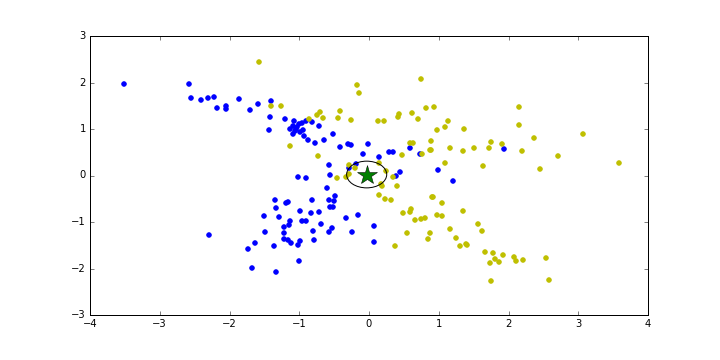
\includegraphics[width=\textwidth]{images/neighborhood.png}
  \end{columns}
\end{frame}

\subsection{Training}
\begin{frame}
  \frametitle{Training}
  \begin{columns}
    \column{0.8\textwidth}
    \includegraphics[width=\textwidth]{images/training_start.png}
  \end{columns}
\end{frame}

\begin{frame}
  \frametitle{Training}
  \begin{columns}
    \column{0.8\textwidth}
    \includegraphics[width=\textwidth]{images/training_end.png}
  \end{columns}
\end{frame}

\subsection{Prediction}
\begin{frame}
  \frametitle{Prediction}
  \begin{enumerate}
    \item Calculate the distance between new points and all points in the training data. \vspace{2mm} \pause
    \item Look at the $k$ points nearest the new point. \vspace{2mm} \pause
    \item Predict the modal class amongst those $k$ points for classification. For regression, choose the average (potentially weighted by distance) of the $k$ points.
  \end{enumerate}
\end{frame}

\subsection{Choosing $k$}
\begin{frame}
  \frametitle{How to Choose $k$}
  \begin{columns}
    \column{1.2\textwidth}
    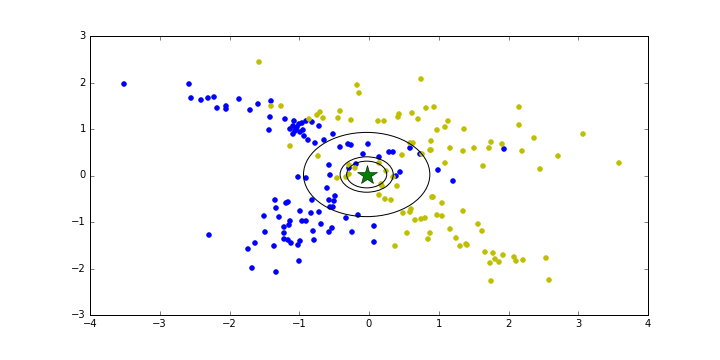
\includegraphics[width=\textwidth]{images/neighborhoods.png}
  \end{columns}
\end{frame}

\begin{frame}
  \frametitle{Bias-Variance Trade-off?}
  \begin{block}{Question}
    How does changing $k$ alter the bias and variance in our $kNN$ models?
  \end{block} \vspace{8mm} \pause
  \begin{columns}
    \column{0.5\textwidth}
    \centering
    What happens when $k=1$? \vspace{4mm} \pause

    $\rightarrow$ {\large High \textcolor{blue}{variance}, low \textcolor{blue}{bias}.} \pause
    \column{0.5\textwidth}
    \centering
    What happens when $k=n$? \vspace{4mm} \pause

    $\rightarrow$ {\large High \textcolor{blue}{bias}, low \textcolor{blue}{variance}.}
  \end{columns}
\end{frame}


\begin{frame}
  \frametitle{$k=1$}
  \begin{columns}
    \column{1.2\textwidth}
    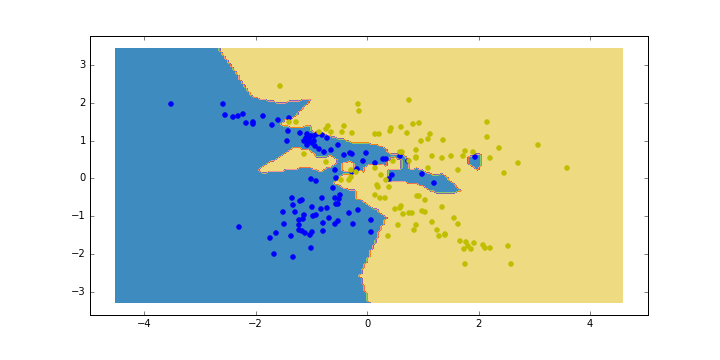
\includegraphics[width=\textwidth]{images/1_neighbors.png}
  \end{columns}
\end{frame}

\begin{frame}
  \frametitle{$k=3$}
  \begin{columns}
    \column{1.2\textwidth}
    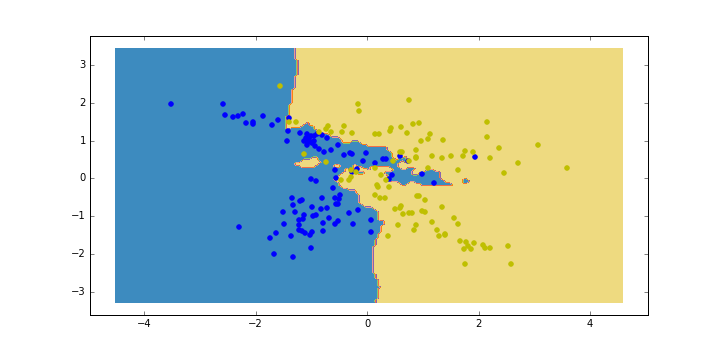
\includegraphics[width=\textwidth]{images/3_neighbors.png}
  \end{columns}
\end{frame}

\begin{frame}
  \frametitle{$k=20$}
  \begin{columns}
    \column{1.2\textwidth}
    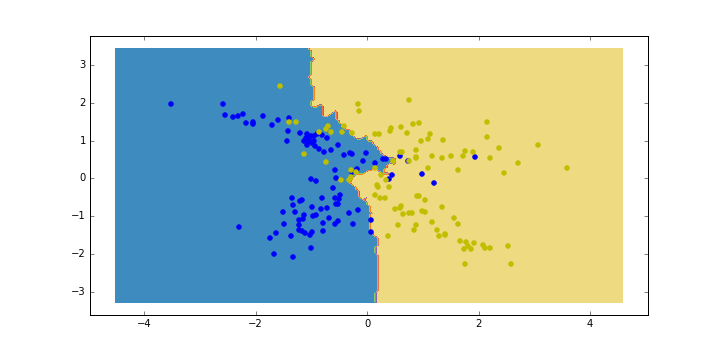
\includegraphics[width=\textwidth]{images/20_neighbors.png}
  \end{columns}
\end{frame}

\begin{frame}
  \frametitle{$k=80$}
  \begin{columns}
    \column{1.2\textwidth}
    \includegraphics[width=\textwidth]{images/80_neighbors.png}
  \end{columns}
\end{frame}

\begin{frame}
  \frametitle{Distance Metrics}
  So far we haven't been explicit about what distance metrics we're using. Some choices: \vspace{4mm}
  \begin{columns}
    \column{0.5\textwidth}
    \begin{description}
      \item[Euclidean] $ \sqrt{\sum_i (a_i - b_i)^2} $ \vspace{2mm}
      \item[Manhattan] $ \sum_i |a_i - b_i| $ \vspace{2mm}
      \item[Cosine] $ 1 - \frac{a \cdot b}{||a|| ||b||} $
    \end{description}
  \end{columns}
\end{frame}

\begin{frame}
  \frametitle{Pros and Cons}
  \begin{columns}
    \column{0.5\textwidth}
    \qquad \underline{\LARGE Pros} \vspace{3mm}
    \begin{itemize}
      \item Simple to use and intuitive.
      \item Extremely fast to train ;)
      \item Doesn't assume anything about the relationship between $X$s and $y$.
    \end{itemize} \pause

    \column{0.5\textwidth}
    \qquad \underline{\LARGE Cons} \vspace{3mm}
    \begin{itemize}
      \item Slow to predict.
      \item Unreliable with high dimensional data.
      \item Doesn't work well with categorical features.
    \end{itemize}
  \end{columns}
\end{frame}

\begin{frame}
  \frametitle{Advice}
  \begin{itemize}
    \item A good place to start searching for $k$ is $\sqrt{n}$. \vspace{2mm}
    \item Make sure to normalize data before training. \vspace{2mm}
    \item Not a widely used algorithm for the reasons we saw above, some potential uses: \vspace{2mm}
      \begin{itemize}
        \item Missing data imputation. \vspace{1mm}
        \item Anomaly detection. \vspace{1mm}
      \end{itemize}
  \end{itemize}
\end{frame}

\begin{frame}
  \frametitle{Variants}
  \begin{itemize}
    \item One variant is to weight the votes by $\frac{1}{d_i}$ so closer points get more weight. \vspace{2mm}
    \item Use for regression, take (optionally, weighted) mean of continuous target rather than vote. \vspace{2mm}
    \item Approximate nearest neighbors, overcomes performance issues.
  \end{itemize}
\end{frame}

\section{Curse of Dimensionality}
\subsection{Completely Unintuitive}
\begin{frame}
  \frametitle{Our Intuition is Lacking}
  The intuition that we have developed as beings living in a spatially 3-dimensional world fails us when we try to reason about how far apart things are in high dimensions. \vspace{4mm}
\end{frame}

\begin{frame}
  \frametitle{Hypercubes}
  \begin{block}{Question}
    Consider a hypercube inside a unit-hypercube. How long would we need to make the side of the smaller hypercube to capture 10\% of the volume of the unit-hypercube?
  \end{block} \vspace{2mm} \pause

  \includegraphics[width=\textwidth]{images/unit_hypercubes.png}
\end{frame}
\begin{frame}
  \frametitle{She's a Witch!}
  \begin{columns}
    \column{1.2\textwidth}
    \includegraphics[width=\textwidth]{images/curse_of_dimensionality.png}
  \end{columns}
\end{frame}

\end{document}
